\documentclass[fleqn]{VRIH2025}

\setlength{\mathindent}{0cm}
\thispagestyle{empty}
\usepackage{array}
\usepackage{booktabs}
\usepackage{enumitem}
\usepackage{float}
\usepackage{graphicx}
\usepackage{longtable}
\usepackage{multirow}
\usepackage{xcolor}
\usepackage{url}
\usepackage{hyperref}

\setlist[itemize]{leftmargin=*}
\setlist[enumerate]{leftmargin=*}
\definecolor{publicationred}{RGB}{170,0,0}
\newcommand{\code}[1]{\texttt{#1}}
\newcolumntype{L}[1]{>{\raggedright\arraybackslash}p{#1}}
\sloppy

\begin{document}

\ensubject{Virtual Reality and Intelligent Hardware}
\qyluntan
\ArticleType{Article}
\Year{}
\Month{}
\Vol{}
\No{}
\DOI{}
\ReceiveDate{}
\RevisedDate{}
\AcceptDate{}

\title{A VR-Headset Visual Pipeline for UAV Pilot Situational Awareness: Combining Geospatial Priors and Semantic Object State in an Unreal Engine Digital Twin}{VR-Headset Visual Pipeline for UAV Teleoperation}

\author[1]{Xabier OLAZ}{}
\author[1]{Daniel ALAEZ}{}
\author[1]{Iker GO\~NI}{}
\author[1,2]{Jes\'us VILLADANGOS}{{jesusv@unavarra.es}}

\AuthorCitation{Xabier OLAZ, Daniel ALAEZ, Iker GO\~NI, Jes\'us VILLADANGOS}

\address[1]{Mathematical Engineering and Computer Science Department, Public University of Navarre, Pamplona, Spain}
\address[2]{Institute of Smart Cities, Public University of Navarre, Spain}

\abstract{Virtual-reality headsets and intelligent hardware enable immersive operator interfaces for unmanned aerial vehicle (UAV) teleoperation. When the communication link is reliable, a live video feed may suffice; however, under variable link conditions—such as delay, reduced bandwidth, intermittent connectivity, or privacy constraints—the pilot can lose spatial awareness of terrain, obstacles, and mission-relevant objects. We present a VR-headset digital-twin visual pipeline in which an Unreal Engine / Cesium geospatial prior provides static scene context while an onboard detector sends semantic object-state updates that are reconstructed as time-stamped, uncertainty-aware actors visible to the pilot through a VR headset. The pipeline architecture—spanning detection ingestion, a state-snapshot service, Unreal/Cesium actor lifecycle, and headset visualization—allows the operator to inspect map-derived context, live detections, stale actors, and uncertainty encodings in a single immersive scene. We validate the complete chain on a real-flight replay: recorded UAV video ingested through a simulated per-frame link with ArduPilot telemetry synchronized by content, a fine-tuned detector (mAP50 0.982), and detected objects reconstructed in the twin as geometric proxy actors. The twin reproduced the logged trajectory within 0.24 m, and the reconstructed position of the validated power-line support fell 4.3 m from its orthophoto ground truth. Semantic telemetry carried the mission at 615.8 kbps as emitted (1.67 Mbps normalized), 84.0\% and 70.4\% below H.264 and H.265 encodings of the same video. Measured detection-to-display latency averaged 38.2 ms (p95 252.9 ms); a bounded display budget places end-to-end updates at about 188 ms mean and 503 ms p95. The display is presented as an auxiliary human-in-the-loop aid for pilot spatial awareness, not as certified detect-and-avoid or a replacement for regulatory safety channels.}

\keywords{Virtual reality; Intelligent hardware; UAV; Digital twin; Geospatial scene reconstruction; Semantic telemetry; Teleoperation; Situational awareness}

\maketitle

\section{Introduction}

Remote UAV operation is a spatial decision-making problem. A pilot or mission operator must reason about aircraft pose, terrain, hazards, people, vehicles, mission targets, visibility, and communication degradation while often relying on a video stream and a map display. Modern video links can be effective under favorable coverage, bandwidth, latency, and codec conditions; this paper does not assume that video is intrinsically inadequate. The problem addressed here is narrower: under variable link conditions (delayed, reduced, or intermittently connected operating states), continuous high-quality low-latency video may be insufficient for reasoning about objects outside the camera's current field of view. 

The central problem is the pilot's need to maintain situation awareness from partial, delayed, heterogeneous, and differently trustworthy evidence. A geospatial map or 3D-tile layer can preserve useful static context, but it does not by itself encode what has changed, what is currently observed, what is stale, or what is uncertain. The scientific gap addressed here is the operator-facing interface for combining a geospatial prior with live semantic state updates: the prior supplies static operating context, while dynamic detections or sensor-derived events update only the entities that are new, moving, changed, uncertain, or absent from the map. The validation burden is to show that this dynamic, uncertainty-aware VR scene supports spatial awareness rather than simply producing an attractive visualization.

Virtual reality and telepresence research provide the conceptual basis for this operator-display problem. Virtual reality can be understood through the dimensions that determine telepresence \cite{steuer1992vr}, while situation awareness includes perception of relevant elements, comprehension of their meaning, and projection of their future status \cite{endsley1995theory}. 

The proposed VR-Headset Visual Pipeline addresses this problem by combining a geospatial prior with live semantic-state updates. The architecture connects the onboard detector to a ground-station service that normalizes and publishes a current state snapshot. Unreal Engine then renders the resulting actors over Cesium geospatial context for an operator wearing a VR headset. The reconstructed scene is an auxiliary operator display in which map-derived context, observed dynamic actors, stale actors, and unobserved space must remain visually and semantically distinguishable.

The main research question is: \textit{Can a VR-equipped UAV operator maintain better spatial awareness of mission-relevant terrain, objects, and changes under constrained communication than with video-only or non-immersive hybrid displays, while preserving explicit visibility of map-derived, observed, stale, or uncertain information?}

The intended contributions are:
\begin{itemize}
    \item Defining a VR-headset-centered operator task model for UAV teleoperation, where a geospatial prior is used to preserve static spatial context, while semantic state updates dynamically represent newly detected or changing entities.
    \item Proposing a VR digital-twin architecture that integrates the VR headset, Unreal Engine, Cesium geospatial prior, and a ground-station service with the onboard detector to combine static maps with live semantic scene reconstruction.
    \item Validating the complete chain through a real-flight replay, which provides measured semantic bandwidth reductions against H.264 and H.265 baselines, alongside sub-metre trajectory fidelity and orthophoto-referenced geospatial accuracy for reconstructed objects.
\end{itemize}

\section{Related Work and Positioning}

The VR-Headset Visual Pipeline sits at the intersection of immersive teleoperation, digital twins, semantic communication, and geospatial visualization. 

\subsection{Immersive Teleoperation and Digital Twins}
Immersive interfaces have been studied to improve operator perception in unmanned-vehicle control \cite{fabris2021immersive, roldan2017multirobot}. Recent work on VR teleoperation has explored visual augmentation of live streams \cite{luo2024visual} and compared 3D visualization and VR display designs for remote monitoring \cite{buchner2025remote}. UAV-specific VR and digital-twin studies include augmented-reality mobile digital twins for wildfire prevention \cite{costa2025ardigitaltwin} and VR-based teleoperation for UAV-manipulator systems \cite{yang2025uavmanipulator}. VRIH has explicitly highlighted the connection between virtual reality, intelligent hardware, and digital twins \cite{lv2022vrihdt, ahmed2022vrihdt}. Broader surveys characterize digital twins as cyber-physical representations requiring data synchronization \cite{jones2020dt, barricelli2019dt, singh2021dt}. Our pipeline differs from these works by focusing on a layered prior-plus-state-update operator scene rather than only viewpoint control or simulated piloting.

\subsection{Geospatial Priors and Semantic Communication}
The geospatial-prior layer is grounded in 3D geospatial visualization practice. The OGC 3D Tiles specification defines an open standard for streaming massive 3D geospatial datasets \cite{ogc2022threedtiles}, making it plausible to use Cesium/Unreal as a static scene prior. To update this prior, instead of transmitting full video, the pipeline sends semantic telemetry: the detected entities and their display-relevant attributes. While this differs from theoretical deep-learning semantic communication systems \cite{luo2022semantic, xie2021semantic, shao2022edgeinference}, it offers an operational reduction in bandwidth by transmitting only task-relevant information.

\subsection{UAV Perception and Variable Link Conditions}
UAV object detection is treated as an upstream perception component \cite{cao2023uavdetection}. Vision-based UAV target geolocation has been extensively studied \cite{barber2006geolocation, hosseinpoor2016geolocation, liu2024multiview}. While modern video links (LTE, WebRTC, 5G) can achieve stable low-latency transmissions under ideal conditions \cite{mohamed2025lteuav, chodorek2025webrtc, duangsuwan2026uocrf}, they still suffer from coverage-capacity trade-offs, handovers, and bandwidth constraints in rural or urban air mobility scenarios \cite{chen2025uamstreaming, chintareddy2026vertical}. The relevant scenario for our visual pipeline is an operator task in which video is available only intermittently or at reduced resolution. While multi-sensor fusion (IR, LiDAR, radar) can improve perception under low visibility \cite{li2025irvisuav, farina2026lidarradar, fercho2026faa_svs}, our current implementation uses YOLO on RGB, integrating other sensors as future work.

\section{System Overview}

\subsection{Operator Scenario}
The target scenario is a UAV mission in which a remote operator needs to monitor terrain, aircraft state, obstacles, or mission objects while communication quality is constrained. The operator wears a VR headset and inspects a synthetic 3D scene containing a geospatial prior, UAV pose, detected entities, freshness indicators, and uncertainty indicators. The proposed display is auxiliary and should be used alongside regulatory control links and operational procedures.

\subsection{Architecture}
The VR-Headset Visual Pipeline is organized around the separation between static scene context and dynamic semantic updates. At initialization, Unreal Engine and Cesium build the map-derived geospatial prior over the designated operating area, while the onboard detection source concurrently publishes dynamic objects to a ground-station ingestion service. This service normalizes their source identity, class, confidence, timestamp, uncertainty, and position into a consistent operator-display representation, and exposes the resulting state as a snapshot that a dedicated telemetry component inside Unreal polls at 5~Hz. On each poll, Unreal reconciles the received entities with the live scene by spawning, updating, marking stale, or despawning semantic actors, so that the VR-equipped operator ultimately perceives the fused geospatial prior and the reconstructed semantic-state layer as a single immersive display.

In the intended live deployment, the UAV streams semantic telemetry and autopilot pose data over a wireless link to the ground station, allowing the pilot to navigate remotely using the VR headset and the reconstructed Unreal/Cesium digital twin without relying on a continuous direct video feed. The validation reported in this paper, however, is a recorded-flight replay over a simulated local link rather than a live field trial.

\begin{figure}[t]
    \centering
    % Placeholder:figura_arquitectura.png
    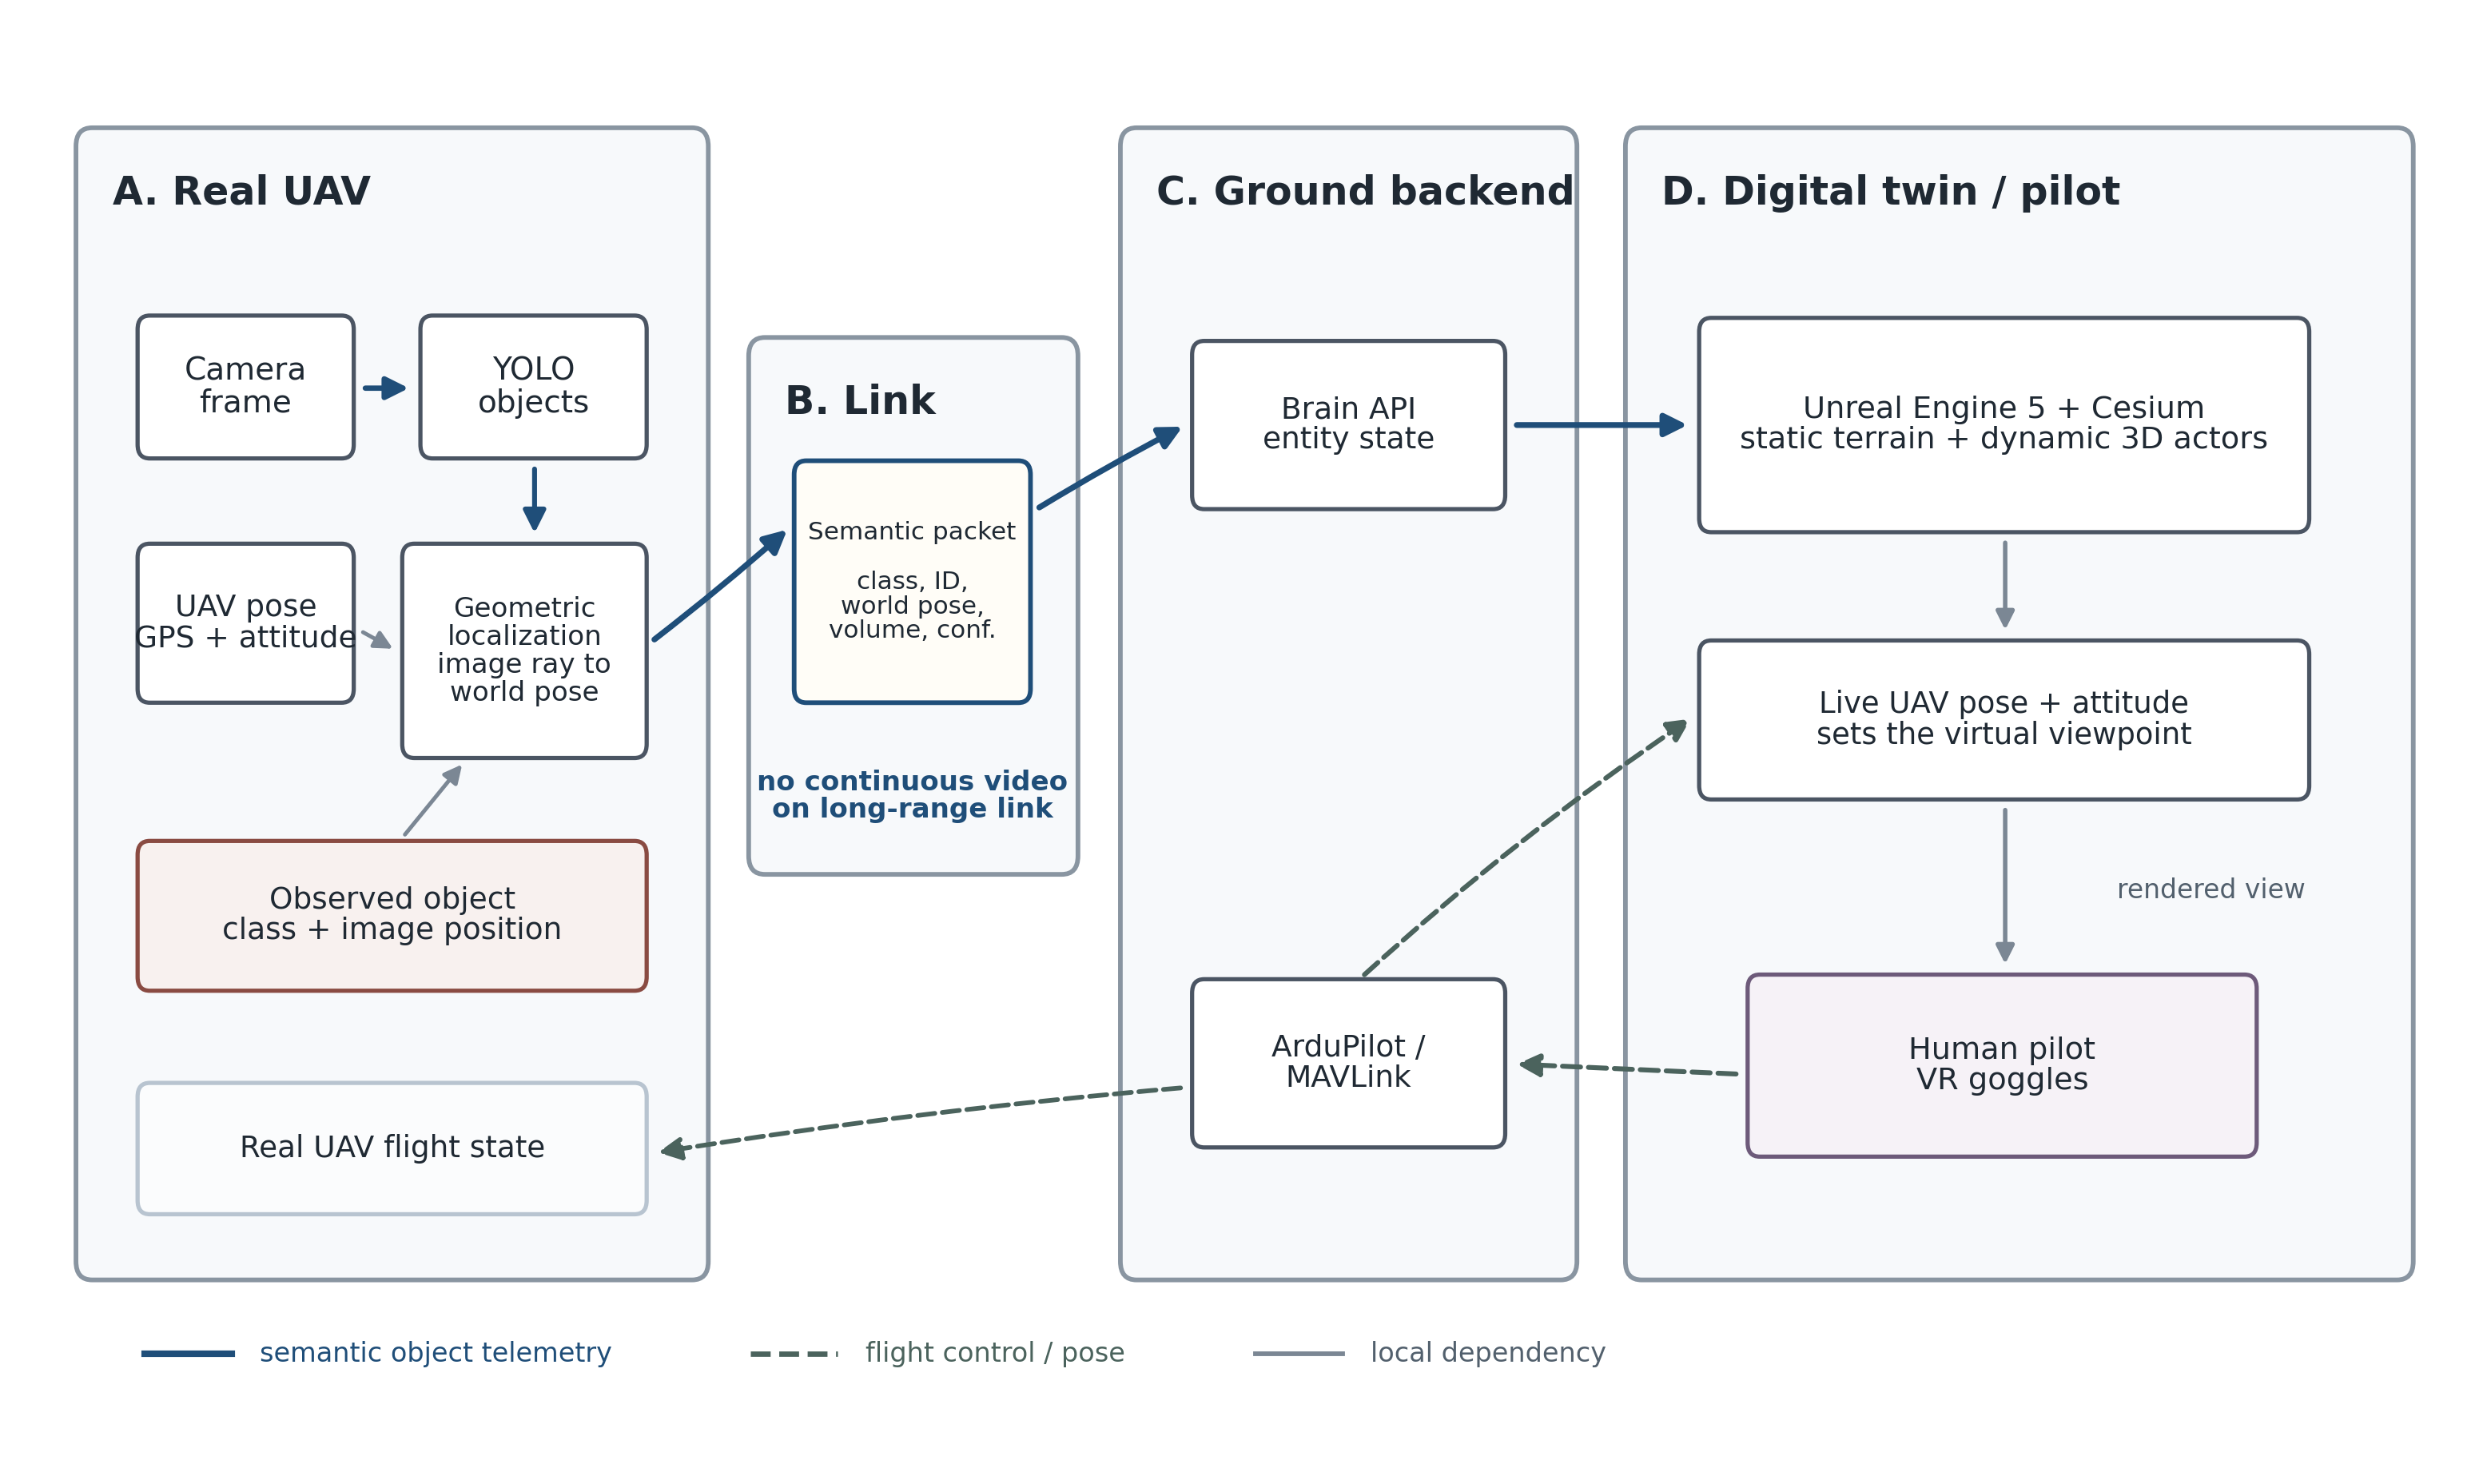
\includegraphics[width=\linewidth]{figures/pipeline_b_architecture.png}
\caption{VR-Headset Visual Pipeline architecture. Cesium and Unreal provide a geospatial prior, while the onboard detector estimates world coordinates and sends semantic state updates to a ground-station service. The service publishes a snapshot to Unreal, which fuses it with autopilot telemetry into an auxiliary VR operator display.}
    \label{fig:pipeline-b-architecture}
\end{figure}

\begin{figure}[t]
    \centering
    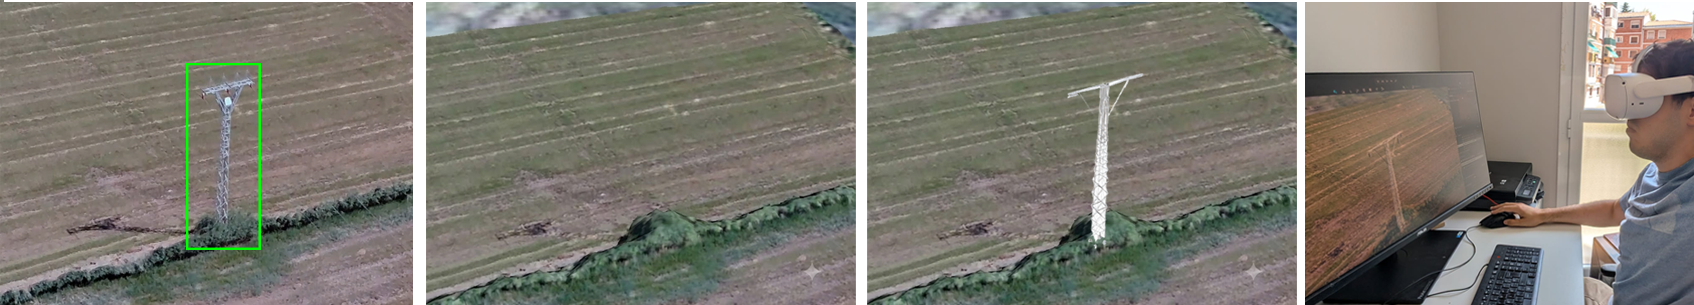
\includegraphics[width=\linewidth]{figures/comparativa.png}
\caption{End-to-end flow of a tower detection. (1) Onboard frame with the YOLO tower bounding box; (2) the semantic state snapshot published by the ground-station service and polled by the Unreal component; (3) the reconstructed tower proxy actor placed in the Unreal/Cesium twin at the georeferenced position; (4) the operator inspecting the scene through the Meta Quest~2 headset. Panels (3) and (4) are shown as placeholders pending the final captures.}
    \label{fig:e2e-pipeline-panels}
\end{figure}

\subsection{Implementation Workflow}
The runtime distinguishes a one-time static-context setup from a continuous dynamic-update loop. Unreal and Cesium initialize the map-derived scene prior once, after which the system enters a publish--normalize--poll cycle: the detection source emits each new observation; the ground-station service normalizes source identity, class, confidence, timestamp, uncertainty, and position into a canonical entity record; and the Unreal telemetry component polls that snapshot at 5~Hz to reconcile the state with the live scene. On every poll, the component spawns newly confirmed actors, updates the pose of tracked ones, demotes those whose age exceeds the configured staleness threshold, and despawns actors whose tracks have expired. This design keeps the heavy geospatial prior on the ground station while the downlink to the operator carries only the semantic delta, which is the basis of the bandwidth advantage reported in Section~\ref{sec:results}.

\begin{table}[H]
\centering
\small
\caption{VR-Headset Visual Pipeline data flow.}
\label{tab:pipeline-b-runtime}
\begin{tabular}{@{}L{0.22\linewidth}L{0.30\linewidth}L{0.34\linewidth}@{}}
\toprule
Stage & Producer & Consumer and required evidence \\
\midrule
Static scene prior & Unreal/Cesium, 3D-tile source & VR-headset runtime; map origin recorded \\
Semantic-state production & YOLOE-26s base (mAP50 0.982) & Telemetry encoder \\
Estimated georeferencing & UAV pose, camera model, terrain & Detection message; mount validated by orthophoto overlay \\
State publication & Ground-station service & Unreal component; 5~Hz polling \\
Actor reconstruction & Unreal component & VR operator display; spawn/update/despawn lifecycle verified \\
Immersive display & Unreal/Cesium runtime & Target HMD: Meta Quest 2 and Quest 3 (informally demonstrated, not formally validated); desktop twin used for this replay \\
\bottomrule
\end{tabular}
\normalsize
\end{table}

\begin{table}[H]
\centering
\small
\caption{Implementation configuration for the desktop digital-twin runtime and target VR headset.}
\label{tab:implementation-config}
\begin{tabular}{@{}L{0.26\linewidth}L{0.62\linewidth}@{}}
\toprule
Component & Configuration \\
\midrule
Game engine & Unreal Engine 5.7 \\
Geospatial prior & Cesium for Unreal (3D Tiles, OGC 22-025r4); operating region pre-cached \\
Ground-station service & Custom state-snapshot service, polled by Unreal at 5~Hz \\
Workstation CPU & AMD Ryzen 9 9950X, 16 cores / 32 threads \\
Workstation GPU & NVIDIA GeForce RTX 5090, 32~GB VRAM (driver 610.62) \\
Workstation memory & 64~GB RAM (62~GB visible to Windows), Windows 11 25H2 \\
Target HMD & Meta Quest 2 (1832$\times$1920 per eye, up to 120~Hz, $\sim$90$^\circ$~H FoV) and Meta Quest 3 (2064$\times$2208 per eye, 72/90/120~Hz, $\sim$110$^\circ$~H FoV) \\
HMD validation status & Informal demonstration only; source-to-photon latency, sustained stereoscopic frame rate, and an operator study are deferred to future work \\
\bottomrule
\end{tabular}
\normalsize
\end{table}

\subsection{Data Representation and Actor Lifecycle}
Each reconstructed object is represented as a display entity:
\begin{equation}
e_i(t) = \{ id_i, c_i, q_i, p_i, \Sigma_i, s_i, a_i, g_i, r_i, m_i \},
\end{equation}
where \(id_i\) is identity, \(c_i\) class, \(q_i\) confidence, \(p_i\) position, \(\Sigma_i\) uncertainty, \(s_i\) source, \(a_i\) age, \(g_i\) geometry, \(r_i\) information role (prior, live, stale), and \(m_i\) metadata. 

The display actor lifecycle is: \text{new} $\rightarrow$ \text{confirmed} $\rightarrow$ \text{updated} $\rightarrow$ \text{stale} $\rightarrow$ \text{removed}. An entity is marked stale when $a_i(t) = t - t_i > \tau_{\mathrm{stale}}$. The replay configuration implements track TTLs of 30~s (static) and 4~s (dynamic).

\subsection{Network Interface and Message Contract}
\label{sec:message-contract}
Unreal does not ingest the raw autopilot stream or the raw detector output. A ground-station service normalizes these two asynchronous sources into a single polled snapshot. The detector publishes detections over a local ingestion interface; the autopilot supplies aircraft state over its telemetry link. The service fuses both, resolves a stable per-object identity, and exposes the operator-display state as a snapshot that the Unreal telemetry component polls at 5~Hz. Each snapshot carries two top-level blocks: a \code{telemetry} object for the UAV and an \code{obstacles[]} array for the reconstructed entities. Table~\ref{tab:message-contract} lists the fields that drive the display; the position is carried both as WGS84 latitude/longitude and as a local ENU \code{world\_m} triple relative to a recorded home origin, and the Unreal component prioritizes \code{world\_m} when present.

\begin{table}[H]
\centering
\small
\caption{Fields of the state snapshot consumed by the Unreal telemetry component.}
\label{tab:message-contract}
\begin{tabular}{@{}L{0.22\linewidth}L{0.18\linewidth}L{0.48\linewidth}@{}}
\toprule
Block / field & Type & Role in the display \\
\midrule
\multicolumn{3}{@{}l}{\textit{telemetry} (UAV state, one per snapshot)} \\
\quad \code{lat}, \code{lon}, \code{alt}, \code{rel\_alt} & float & Geodetic position of the aircraft \\
\quad \code{world\_m.\{north,east,up\}} & float & Local ENU position relative to home; preferred by Unreal \\
\quad \code{yaw}, \code{heading} & deg & Aircraft heading (used for actor orientation) \\
\quad \code{mode}, \code{armed}, \code{groundspeed} & mixed & Flight-mode, arm state, and ground speed context \\
\midrule
\multicolumn{3}{@{}l}{\textit{obstacles[i]} (reconstructed entity, one per detected object)} \\
\quad \code{entity\_id}, \code{object\_id} & string & Stable identity for spawn/update/despawn lifecycle \\
\quad \code{type}, \code{object\_type} & string & Canonical class label (e.g.\ \textit{tower}, \textit{cow}, \textit{bike}) \\
\quad \code{world\_m.\{north,east,up\}} & float & Local ENU position; preferred by Unreal when present \\
\quad \code{lat}, \code{lon} & float & Geodetic fallback for position \\
\quad \code{confidence} & 0--1 & Detection confidence; drives confirmed/stale demotion \\
\quad \code{yaw\_deg}, \code{heading\_deg} & deg & Optional object heading \\
\quad \code{track\_age\_s}, \code{track\_seen\_count}, \code{track\_static} & mixed & Freshness and static/dynamic track metadata (TTL selection) \\
\bottomrule
\end{tabular}
\normalsize
\end{table}

\section{Method}

\subsection{Layered Scene-State Model}
At time \(t\), the operator display is modeled as a layered scene state:
\begin{equation}
S(t) = \{G_0(\Omega), x_u(t), E_{\Delta}(t), U(t), H(t)\},
\end{equation}
where \(G_0(\Omega)\) is the geospatial prior, \(x_u(t)\) is UAV state, \(E_{\Delta}(t)\) is the set of semantic updates, \(U(t)\) contains uncertainty/freshness annotations, and \(H(t)\) denotes the VR-headset view. This model allows the system to remain useful when live video is degraded: the display is not blank because \(G_0(\Omega)\), \(x_u(t)\), and the last validated \(E_{\Delta}(t)\) provide bounded spatial context.

\subsection{Detection-to-World Projection}
The georeferencing step estimates world coordinates using explicit camera, pose, and terrain assumptions. A detector returns a bounding box \(b=[x_1,y_1,x_2,y_2]^T\), and the projected ground-contact pixel is the bottom-centre point:
\begin{equation}
z_b = \begin{bmatrix} u_b \\ v_b \end{bmatrix} = \begin{bmatrix} (x_1+x_2)/2 \\ y_2 \end{bmatrix}.
\end{equation}
Using a pinhole approximation from image size \(W\times H\) and vertical FOV \(\psi_v\), the normalized camera-frame ray for \(z_b\) is mapped to the UAV body frame and then to local North--East--Down (NED) using UAV yaw, pitch, and roll. With NED down positive and UAV height \(h\), the ground-plane intersection yields North/East offsets:
\begin{equation}
t_b = \frac{h}{r_{n,D}}, \quad N=t_b r_{n,N}, \quad E=t_b r_{n,E}, \quad d_h=\sqrt{N^2+E^2}.
\end{equation}
For the Unreal/Cesium runtime, this estimate is expressed in a local tangent frame and published as \code{world\_m}. This projection is sensitive to bounding-box choice, camera calibration, and timestamp synchronization; therefore, the projected position is an estimate, not a proof of target location.

\subsection{Semantic Telemetry Bandwidth}
For a mission interval \(T\), with \(N\) entity messages of size \(|m_k|\) bytes, semantic telemetry bitrate is:
\begin{equation}
B_{\mathrm{sem}} = \frac{8}{T}\sum_{k=1}^{N} |m_k|.
\end{equation}
The total display traffic is \(B_{\mathrm{display}} = B_{\mathrm{pose}} + B_{\Delta} + B_{\mathrm{prior}}\). If the operating area is pre-cached, \(B_{\mathrm{prior}}\) is near zero. The bandwidth reduction against a video baseline is \(\Delta B = (B_{\mathrm{video}} - B_{\mathrm{sem}}) / B_{\mathrm{video}}\).

\subsection{Latency Decomposition}
End-to-end latency from source event to visible update in the VR headset is:
\begin{equation}
L_{\mathrm{e2e}} = L_{\mathrm{det}} + L_{\mathrm{uplink}} + L_{\mathrm{svc}} + L_{\mathrm{poll}} + L_{\mathrm{actor}} + L_{\mathrm{render}} + L_{\mathrm{vr}}.
\end{equation}
The software-only segments can be instrumented immediately. The complete source-to-VR-headset measurement requires the Unreal VR runtime and the operator's VR headset.

\section{Results: Real-Flight Replay Validation}
\label{sec:results}

\subsection{Replay Setup and Synchronization}
The validation uses a recorded power-line inspection flight (M\_20\_1RR). The onboard video was processed into an analysis segment (1280$\times$960, 10~fps) and synchronized to the autopilot log by content matching against the recorded frames. A tower detector fine-tuned from a YOLOE-26s base reaches mAP50 0.982. Detected supports are georeferenced, tracked by the ground-station service, and reconstructed as proxy actors.

\begin{figure}[t]
    \centering
    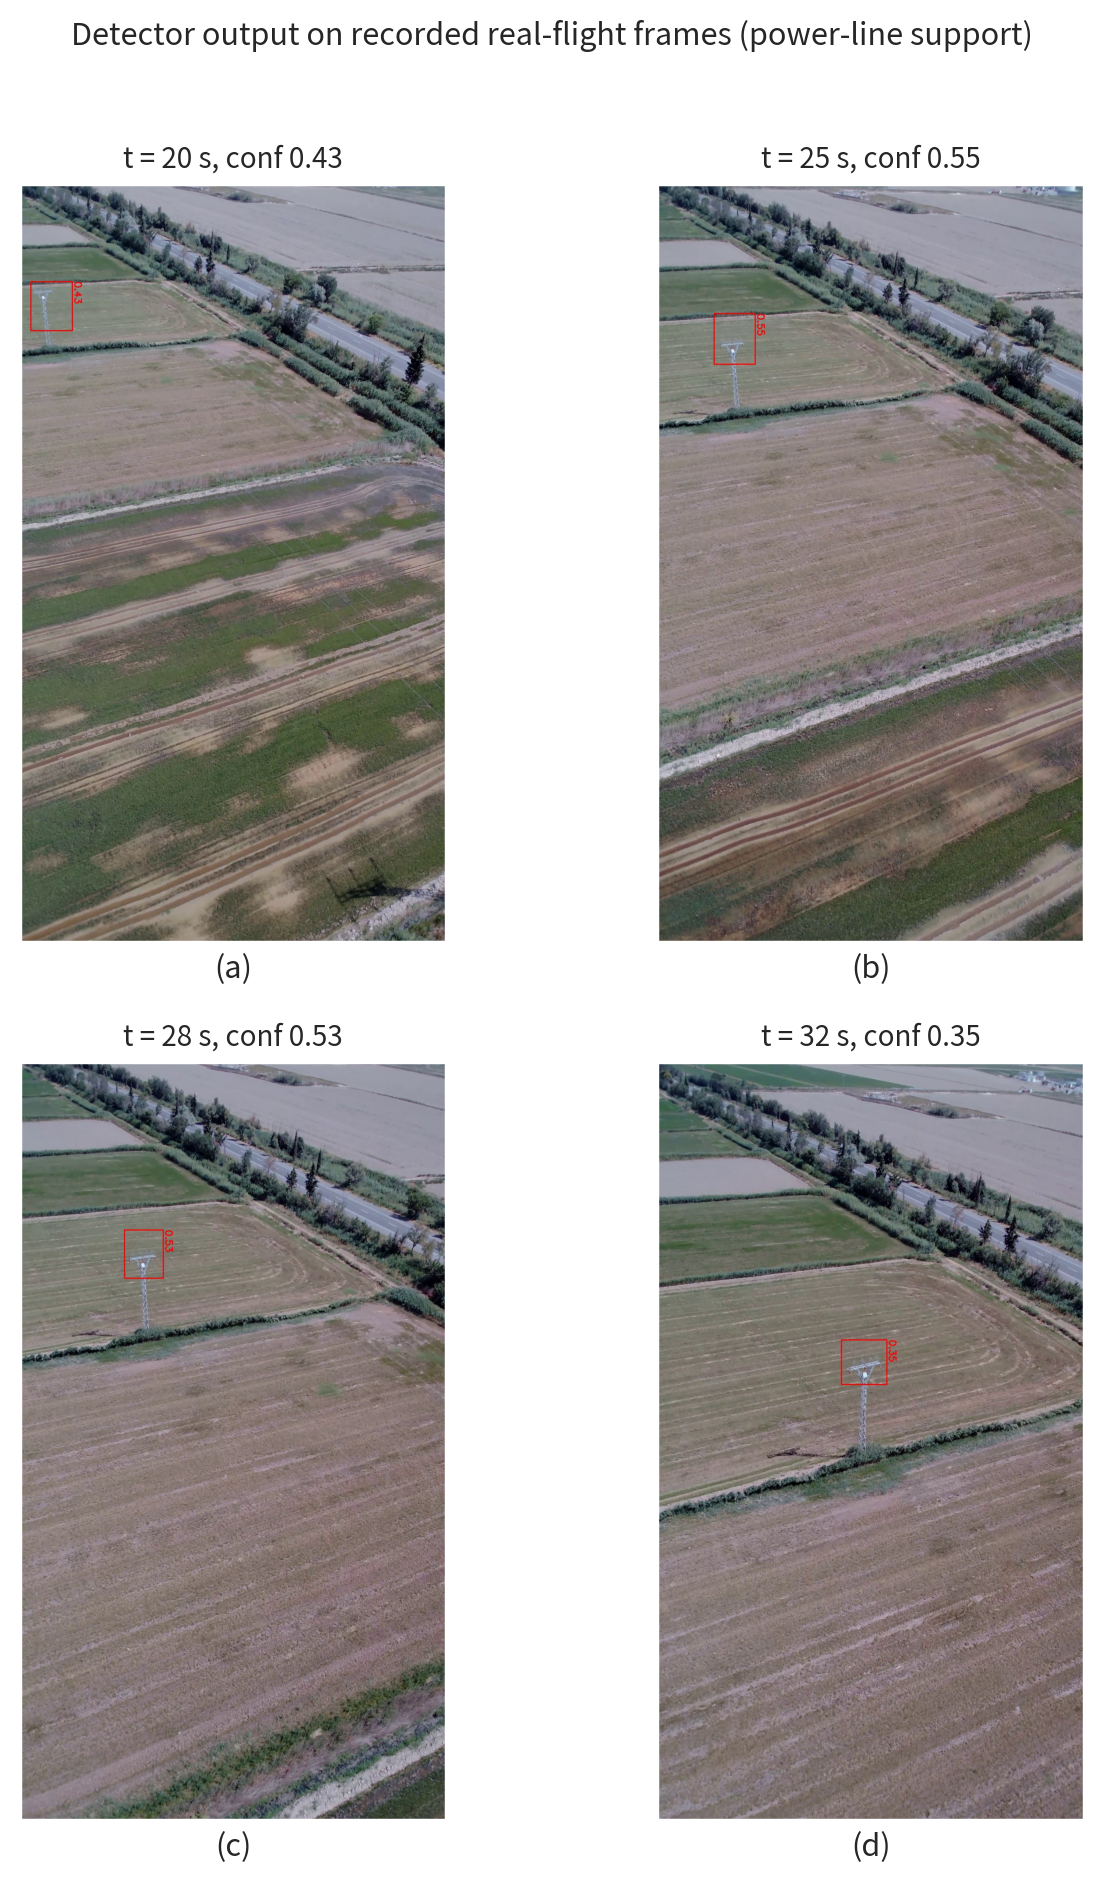
\includegraphics[width=0.82\linewidth]{figures/fig_detection_grid.png}
\caption{Detector output on four recorded frames of the real-flight segment.}
    \label{fig:detection-grid}
\end{figure}

\subsection{Semantic Bandwidth versus Video Baselines}
Over the replayed mission, the detector published 554 obstacle messages totalling 14.46~MB. Normalized to the 69.2~s mission interval, the stream corresponds to 1.67~Mbps. Baselines were encoded from the same flight video: H.264 at 10.43~Mbps and H.265 at 5.65~Mbps. The mission-normalized reduction is 84.0\% against H.264 and 70.4\% against H.265. These figures exclude Cesium tile traffic, as the operating region was pre-cached.

\begin{figure}[t]
    \centering
    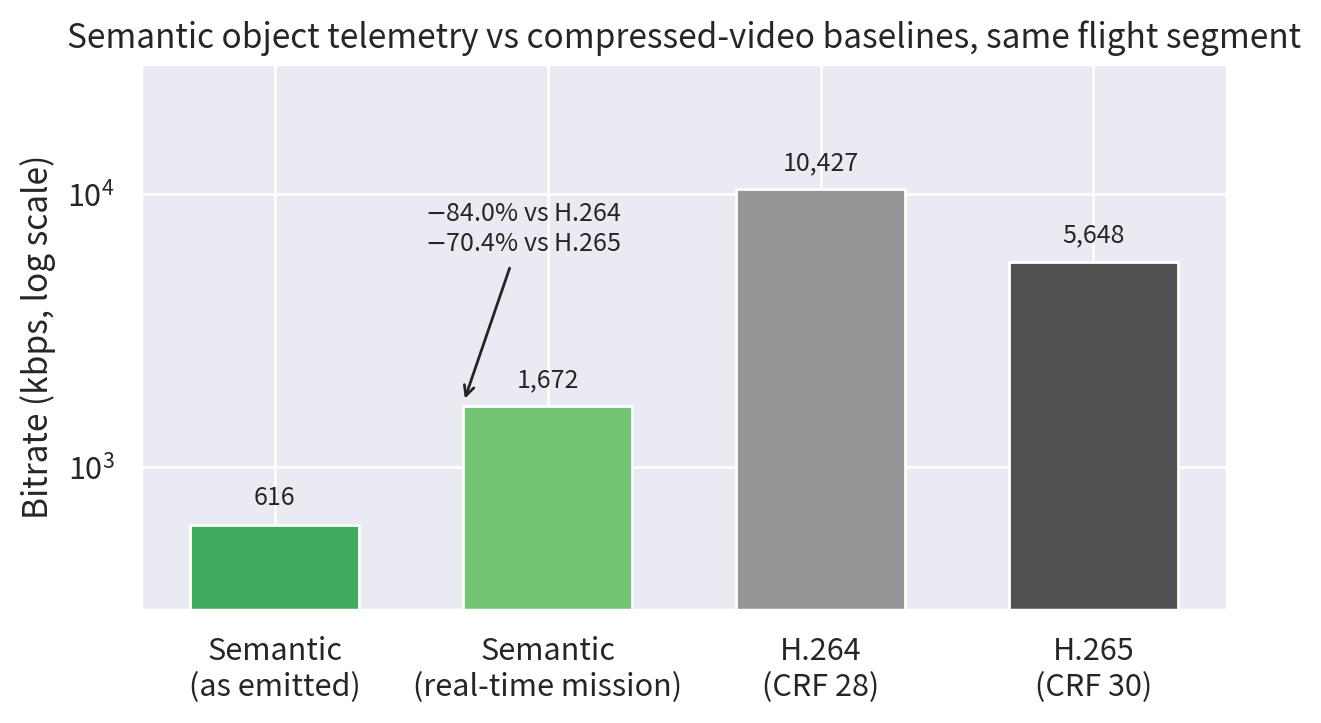
\includegraphics[width=0.9\linewidth]{figures/fig_bandwidth.png}
\caption{Bitrate of the semantic object-telemetry stream against H.264 and H.265 encodings.}
    \label{fig:bandwidth}
\end{figure}

\subsection{Latency}
The measured detection-to-display latency averages 38.2~ms with a p95 of 252.9~ms. Adding a conservative display budget for the remaining software segments (5~Hz poll and 50~ms actor spawn/render) bounds the end-to-end update latency at about 188~ms mean and 503~ms p95 for a visible proxy update in the desktop twin. This figure excludes HMD presentation latency.

\begin{figure}[t]
    \centering
    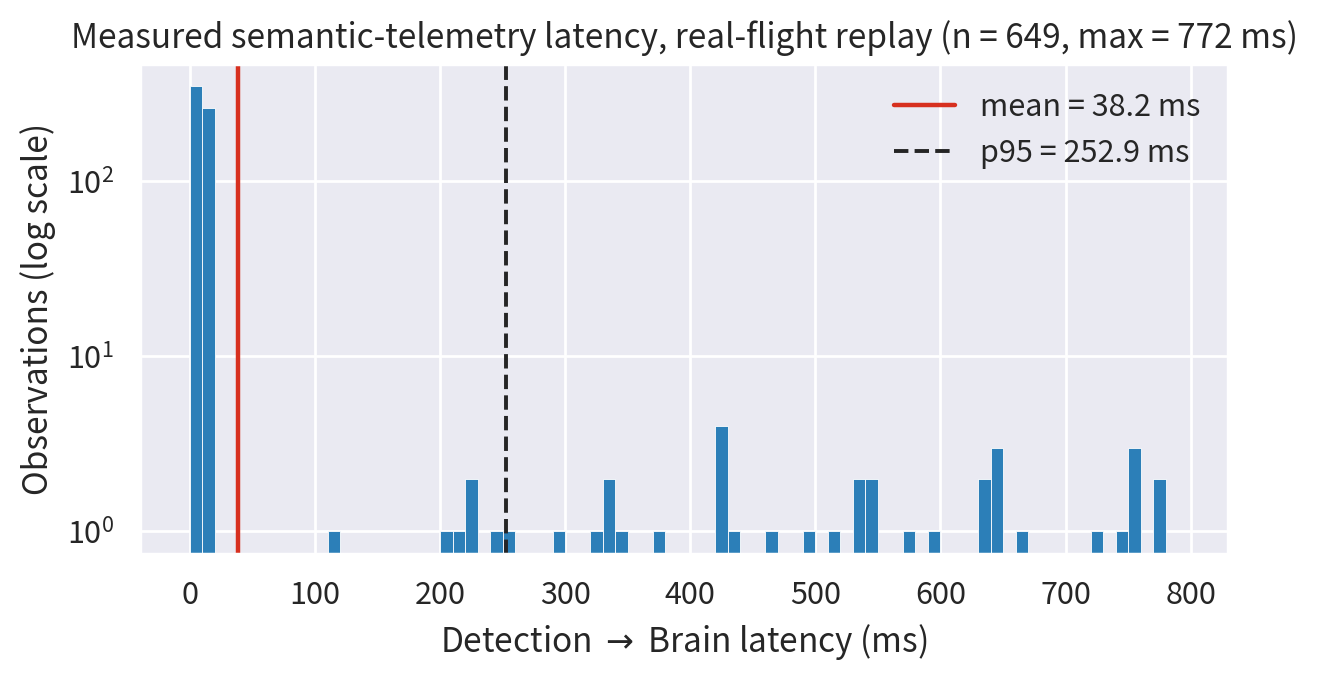
\includegraphics[width=0.9\linewidth]{figures/fig_latency_hist.png}
\caption{Measured detection-to-display latency for the 649 detection records.}
    \label{fig:latency-hist}
\end{figure}

\subsection{Trajectory Fidelity and Geospatial Accuracy}
The twin aircraft was driven by the service-published world positions. Against the reference trajectory, the commanded path shows a cross-track error of 0.24~m maximum ($n=2363$). Ground truth for power-line supports was marked on PNOA orthophotos. A robust cluster analysis places the main cluster (216 observations, support P3) at 4.3~m from its orthophoto position; the end-to-end georeferencing error is approximately 4--5~m for the validated support at 40--130~m range. Residual error sources: camera-mount residual (2--8~m) and video--log synchronization (8--12~m along track).

\begin{figure}[t]
    \centering
    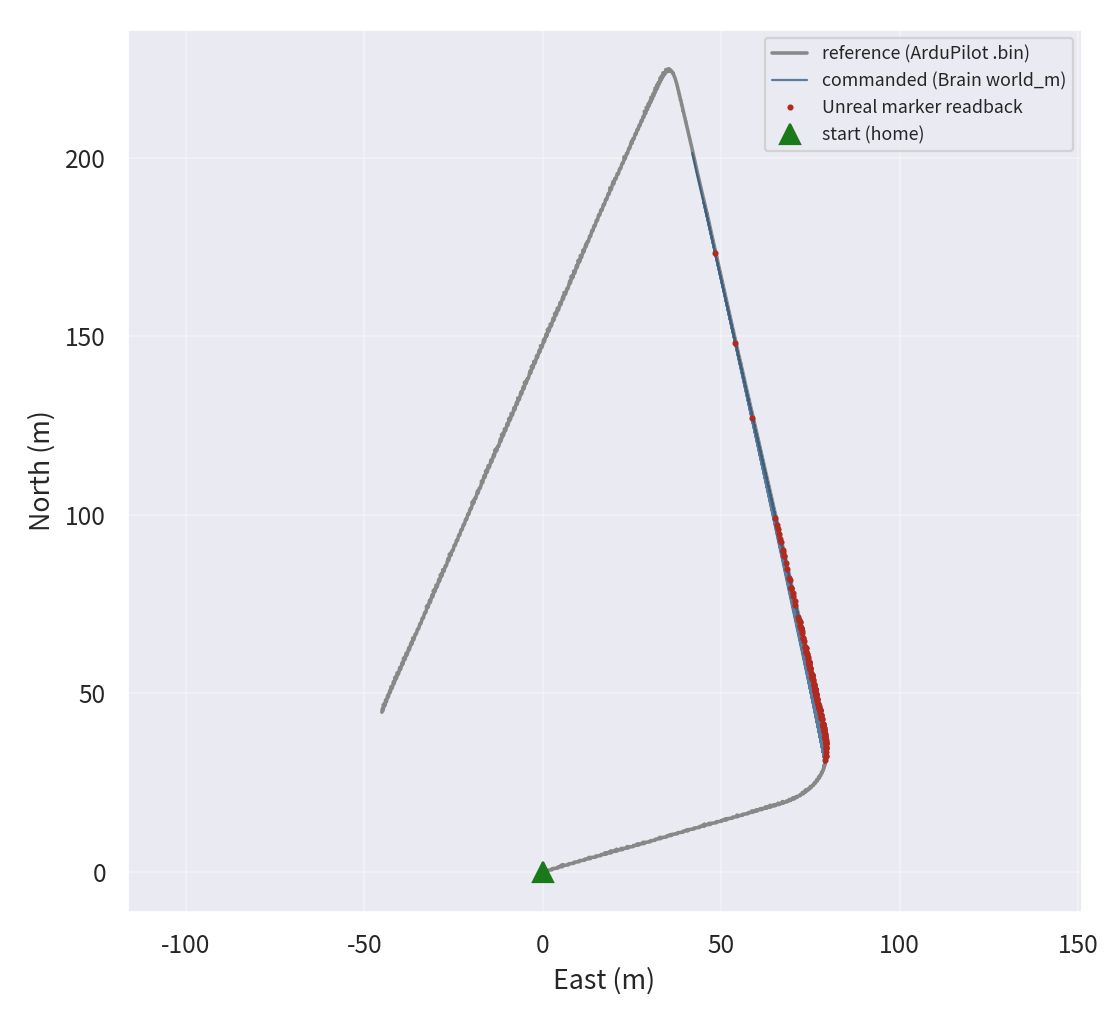
\includegraphics[width=\linewidth]{figures/fig_trajectory_check.png}
\caption{Trajectory fidelity: reference path, service-commanded positions, and Unreal readback.}
    \label{fig:trajectory-check}
\end{figure}

\begin{figure}[t]
    \centering
    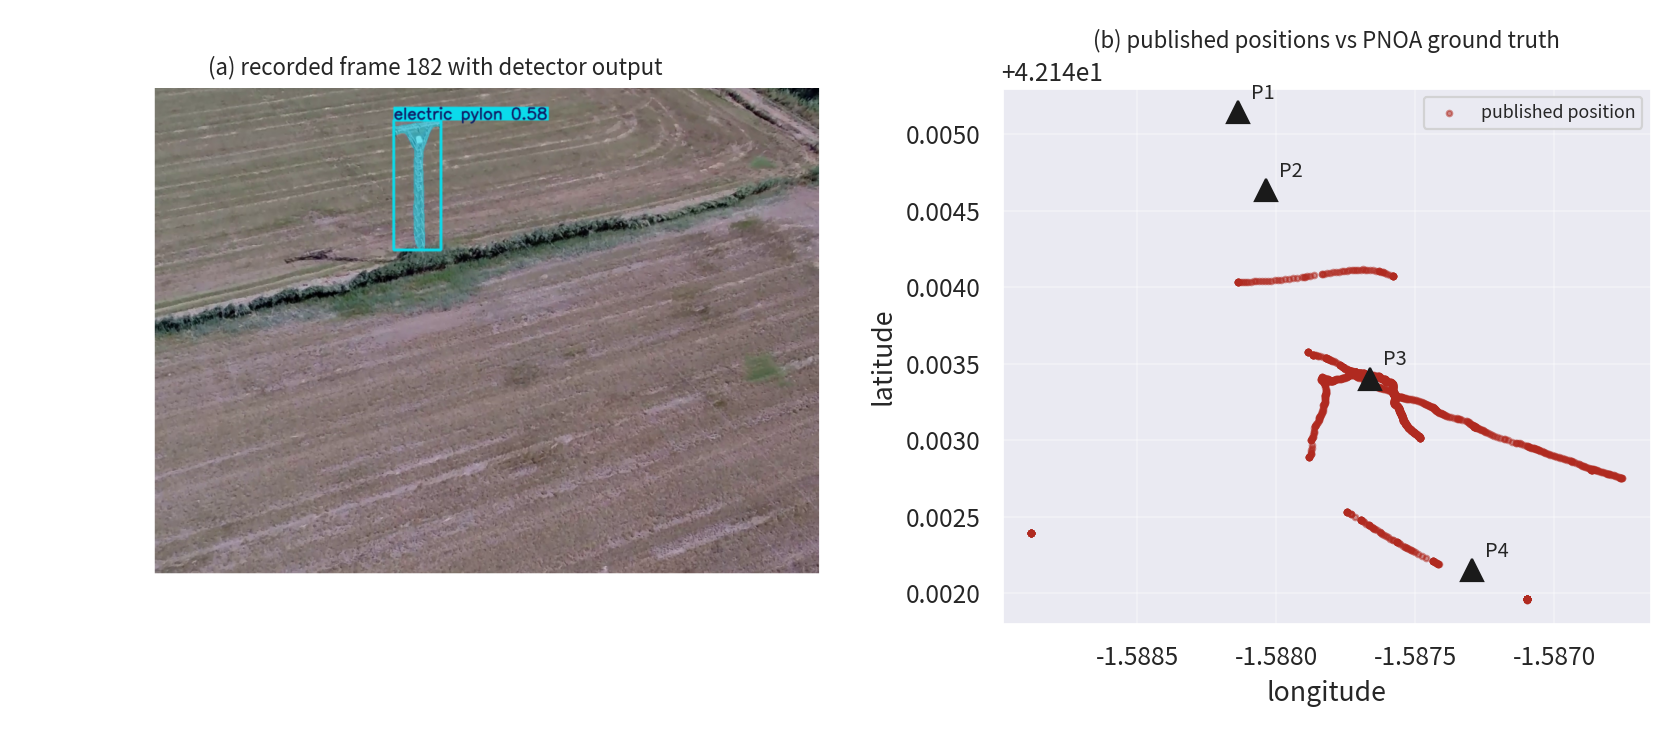
\includegraphics[width=\linewidth]{figures/fig_real_vs_map.png}
\caption{Real detection and geospatial validation against PNOA orthophoto ground truth.}
    \label{fig:real-vs-map}
\end{figure}

\subsection{Desktop Render Performance}
\label{sec:render-performance}
To confirm that the desktop twin can host the Cesium geospatial prior together with the reconstructed semantic actors without becoming frame-bound, we measured the engine on the workstation listed in Table~\ref{tab:implementation-config} (AMD Ryzen~9 9950X, RTX~5090, 64~GB RAM). The benchmark replayed synthetic obstacle payloads through the same ingestion path used at runtime and reported per-phase frame time (p50/p95) together with estimated component, triangle, and draw-call counts.

Across the measured scene sizes, the create, pose-stream, and shape-stream phases stayed below a 33.3~ms (30~FPS) p95 budget up to 100 reconstructed semantic-proxy actors, while the Unreal CSV profiler reported a global \code{GPUTime} p50/p95 of 1.46/1.67~ms and \code{FrameTime} p50/p95 of 4.66/6.32~ms on the lighter global workload. Table~\ref{tab:render-performance} summarizes the per-phase frame time of the actor-level semantic-proxy backend. The 100-object pose- and shape-update streams exceeded a 16.7~ms (60~FPS) p95 budget (17.8~ms and 19.3~ms respectively), which bounds the dense-scene update rate but leaves single-frame rendering headroom on this hardware. These measurements are non-stereoscopic desktop measurements; they establish a smooth desktop baseline for the geospatial prior and dynamic actors and do not constitute VR-headset frame-rate validation.

\begin{table}[H]
\centering
\small
\caption{Desktop render benchmark, semantic-proxy backend, frame-time p95 in milliseconds (Unreal 5.7, RTX~5090).}
\label{tab:render-performance}
\begin{tabular}{@{}L{0.12\linewidth}L{0.12\linewidth}L{0.12\linewidth}L{0.12\linewidth}L{0.14\linewidth}L{0.10\linewidth}@{}}
\toprule
Actors & Create p95 & Pose p95 & Shape p95 & Components / draw calls & Est. triangles \\
\midrule
10  & 4.67 & 4.38 & 4.75 & 44 / 44 & 23\,760 \\
50  & 5.13 & 9.27 & 9.88 & 216 / 216 & 104\,432 \\
100 & 4.82 & 17.81 & 19.26 & 432 / 432 & 208\,864 \\
\bottomrule
\end{tabular}
\normalsize
\end{table}

\subsection{Degradation Profiles}
Network degradation was simulated using loss and jitter profiles: visible-entity recall was 0.949 under 5\% loss with 50~ms jitter and 0.843 under 15\% loss with 200~ms jitter. The actor lifecycle behaved as specified: proxy actors spawn on detection, persist through tracked updates, are demoted when stale, and despawn on track expiry.

\subsection{HMD Recognition Feasibility}
\label{sec:hmd-feasibility}
As a preliminary feasibility check (not a controlled validation), one operator wearing a Meta Quest~2 headset (Table~\ref{tab:implementation-config}) could visually identify the reconstructed semantic actors of the three canonical classes used in the workflow---power-line supports (\textit{tower}), livestock (\textit{cow}), and vehicles/bicycles (\textit{bike})---from the semantic state stream alone, without any video feed. The proxy actors reconstructed by Unreal were discriminable in the immersive view against the Cesium geospatial prior. This observation is reported as perceptual feasibility only: it involves a single operator, no baseline condition (video-only, prior-only, non-immersive hybrid), and no workload instrument, so it does not establish operator benefit. Its role is to motivate, not to substitute for, the controlled operator study defined as future work (Section~\ref{sec:discussion}).

\section{Limitations and Safety Envelope}

The VR-Headset Visual Pipeline can mislead an operator if uncertainty is hidden, and several limitations are inherent to the system definition. On the semantic side, an absent actor may denote an undetected object rather than safe empty space, and a stale actor can retain an authoritative appearance unless its age, source, and confidence are visibly demoted in the display. On the geospatial side, the prior can be outdated, omit temporary obstacles such as cables, and accumulate placement errors whenever terrain or coordinate systems are misaligned; the measured 4--5~m error therefore bounds the display to spatial-awareness support rather than precision maneuvering.

The communication advantage itself rests on a pre-cached operating region, since streaming geospatial tiles over the same constrained link would erode the bandwidth reduction. The immersive interface additionally inherits the human-factor risks common to VR, including cybersickness, attentional tunneling, fatigue, and display occlusion. From a regulatory standpoint, Beyond Visual Line of Sight operation requires certified detect-and-avoid and command-and-control reliability that an auxiliary display of this kind cannot provide.

The validation reported here is deliberately bounded: it covers a single flight, a single scenario, a single object class, and a simulated local link, so generalization will require additional flights and real radio measurements. Real-time onboard performance is likewise not established; the separate non-stereoscopic desktop render benchmark (Section~\ref{sec:render-performance}) confirms only that the engine hosts the geospatial prior and up to 100 reconstructed actors below a 30~FPS p95 frame budget, which is not VR-headset frame-rate evidence.

The safety envelope operationalizes these constraints through bounded stale-object age (a track TTL of 30~s for static entities and 4~s for dynamic ones), a maximum position-uncertainty radius, a minimum detection confidence, fallback rules that visually demote actors on staleness and despawn them on expiry, and an explicit prohibition against using the display as a certified detect-and-avoid channel.

\section{Discussion and Future Work}
\label{sec:discussion}

The proposed system's effectiveness depends on several validity requirements. First, spatial awareness must be measured through task performance and established human-factor instruments (such as NASA-TLX or SAGAT) rather than inferred from visual plausibility. Second, baseline parity between video-only, prior-only, non-immersive hybrid, and VR digital-twin conditions is essential. Third, the VR-headset scene must be strictly tied to logs, timestamps, and ground truth.

This structure makes the core hypothesis falsifiable. The pipeline is supported only if the VR digital-twin condition improves or preserves task-relevant spatial awareness under constrained communication without unacceptable increases in workload or overtrust. The strongest version of the contribution is that a VR operator display can explicitly combine prior scene knowledge and live semantic state updates in a way that remains inspectable under degraded video.

\textbf{Future Work:} The immediate next steps include VR-headset capture with source-to-photon latency measurement, a hardware-in-the-loop campaign with a live autopilot, field measurements over a real degraded radio link, completion of the corridor ground-truth map, and a controlled operator study to measure human utility and workload.

\section{Conclusion}

The VR-Headset Visual Pipeline is presented as a human-in-the-loop digital-twin operator display for UAV teleoperation. The implemented workflow uses Unreal/Cesium as a bounded geospatial prior, converts detected changes into semantic telemetry, publishes a live entity snapshot through the ground-station service, and reconstructs dynamic actors inside a VR-headset-visible scene. The publishable contribution is that the integrated VR-headset scene layer can be specified, instrumented, and evaluated as an operator aid for spatial awareness when video-only displays may be insufficient. The stored-flight replay validation confirms content-synchronized video and telemetry, detection at mAP50 0.982, semantic telemetry at 1.67~Mbps mission-normalized (84.0\% and 70.4\% below H.264 and H.265), detection-to-display latency of 38.2~ms mean, sub-metre trajectory fidelity, and a 4.3~m geospatial error against orthophoto ground truth.

\section*{Acknowledgements}
The authors thank the Institute of Smart Cities (Public University of Navarre) for institutional support.

\section*{CRediT Author Statement}
\textbf{Xabier Olaz}: Conceptualization, Methodology, Software, Investigation, Writing -- original draft. \textbf{Daniel Alaez}: Software, Validation, Data curation. \textbf{Iker Go\~ni}: Software, Validation, Data curation. \textbf{Jes\'us Villadangos}: Supervision, Writing -- review \& editing, Project administration.

\section*{Declaration of Competing Interest}
The authors declare that they have no known competing financial interests or personal relationships that could have appeared to influence the work reported in this paper.

\section*{Data and Code Availability}
The replay artifacts, audit logs, sealed JSON/CSV metrics, and analysis scripts that support the results of this paper are part of the project repository. The recorded flight video and autopilot logs are available from the corresponding author upon reasonable request.

\section*{Ethics Statement}
This study did not involve human subjects or animals; the operator study defined as future work will be submitted for ethics review before recruitment.

\section*{Declaration of Generative AI and AI-Assisted Technologies}
During the preparation of this work the authors used AI-assisted tools for language editing and code assistance. The authors reviewed and edited all content and take full responsibility for the integrity of the publication.

\begin{thebibliography}{60}

\bibitem{steuer1992vr}
Steuer J. Defining virtual reality: Dimensions determining telepresence. Journal of Communication, 1992, 42(4): 73--93. doi: \url{https://doi.org/10.1111/j.1460-2466.1992.tb00812.x}

\bibitem{endsley1995theory}
Endsley M R. Toward a theory of situation awareness in dynamic systems. Human Factors, 1995, 37(1): 32--64. doi: \url{https://doi.org/10.1518/001872095779049543}

\bibitem{fabris2021immersive}
Fabris E J, Sangalli V A, Soares L P, et al. Immersive telepresence on the operation of unmanned vehicles. International Journal of Advanced Robotic Systems, 2021, 18(1). doi: \url{https://doi.org/10.1177/1729881420978544}

\bibitem{roldan2017multirobot}
Rold\'an J, Pe\~na-Tapia E, Mart\'in-Barrio A, et al. Multi-robot interfaces and operator situational awareness: Study of the impact of immersion and prediction. Sensors, 2017, 17(8): 1720. doi: \url{https://doi.org/10.3390/s17081720}

\bibitem{luo2024visual}
Luo Y, Wang J, Pan Y, et al. Visual augmentation of live-streaming images in virtual reality to enhance teleoperation of unmanned ground vehicles. Frontiers in Virtual Reality, 2024, 5. doi: \url{https://doi.org/10.3389/frvir.2024.1230885}

\bibitem{buchner2025remote}
Buchner S L, Rindfuss A, Wood J, et al. Impacts of 3D visualizations and virtual reality in display designs for remote monitoring of satellite operations. Frontiers in Virtual Reality, 2025, 6. doi: \url{https://doi.org/10.3389/frvir.2025.1487281}

\bibitem{costa2025ardigitaltwin}
Costa C, Gomes E, Rodrigues N, et al. Augmented reality mobile digital twin for unmanned aerial vehicle wildfire prevention. Virtual Reality, 2025, 29(2). doi: \url{https://doi.org/10.1007/s10055-025-01145-w}

\bibitem{yang2025uavmanipulator}
Yang Z, Tomita K, Kamimura A. VR-based teleoperation of UAV--manipulator systems: From single-UAV control to dual-UAV cooperative manipulation. Applied Sciences, 2025, 15(20): 11086. doi: \url{https://doi.org/10.3390/app152011086}

\bibitem{lv2022vrihdt}
Lv Z, Marfia G, Poiesi F, et al. Virtual-reality and intelligent hardware in digital twins. Virtual Reality \& Intelligent Hardware, 2022, 4(4): ii--iv. doi: \url{https://doi.org/10.1016/j.vrih.2022.08.002}

\bibitem{ahmed2022vrihdt}
Ahmed I, Ahmad M, Jeon G. Integrating digital twins and deep learning for medical image analysis in the era of COVID-19. Virtual Reality \& Intelligent Hardware, 2022, 4(4): 292--305. doi: \url{https://doi.org/10.1016/j.vrih.2022.03.002}

\bibitem{jones2020dt}
Jones D, Snider C, Nassehi A, et al. Characterising the digital twin: A systematic literature review. CIRP Journal of Manufacturing Science and Technology, 2020, 29: 36--52. doi: \url{https://doi.org/10.1016/j.cirpj.2020.02.002}

\bibitem{barricelli2019dt}
Barricelli B R, Casiraghi E, Fogli D. A survey on digital twin: Definitions, characteristics, applications, and design implications. IEEE Access, 2019, 7: 167653--167671. doi: \url{https://doi.org/10.1109/ACCESS.2019.2953499}

\bibitem{singh2021dt}
Singh M, Fuenmayor E, Hinchy E, et al. Digital twin: Origin to future. Applied System Innovation, 2021, 4(2): 36. doi: \url{https://doi.org/10.3390/asi4020036}

\bibitem{ogc2022threedtiles}
Cozzi P, Lilley S, et al., eds. 3D Tiles Specification. OGC Community Standard 22-025r4, Open Geospatial Consortium, 2022. Available at: \url{https://docs.ogc.org/cs/22-025r4/22-025r4.html}

\bibitem{luo2022semantic}
Luo X, Chen H H, Guo Q. Semantic communications: Overview, open issues, and future research directions. IEEE Wireless Communications, 2022, 29(1): 210--219. doi: \url{https://doi.org/10.1109/MWC.101.2100269}

\bibitem{xie2021semantic}
Xie H, Qin Z, Li G Y, et al. Deep learning enabled semantic communication systems. IEEE Transactions on Signal Processing, 2021, 69: 2663--2675. doi: \url{https://doi.org/10.1109/TSP.2021.3071210}

\bibitem{shao2022edgeinference}
Shao J, Mao Y, Zhang J. Learning task-oriented communication for edge inference: An information bottleneck approach. IEEE Journal on Selected Areas in Communications, 2022, 40(1): 197--211. doi: \url{https://doi.org/10.1109/JSAC.2021.3126087}

\bibitem{cao2023uavdetection}
Cao Z, Kooistra L, Wang W, et al. Real-time object detection based on UAV remote sensing: A systematic literature review. Drones, 2023, 7(10): 620. doi: \url{https://doi.org/10.3390/drones7100620}

\bibitem{barber2006geolocation}
Barber D B, Redding J D, McLain T W, et al. Vision-based target geo-location using a fixed-wing miniature air vehicle. Journal of Intelligent and Robotic Systems, 2006, 47(4): 361--382. doi: \url{https://doi.org/10.1007/s10846-006-9088-7}

\bibitem{hosseinpoor2016geolocation}
Hosseinpoor H R, Samadzadegan F, Dadrasjavan F. Precise target geolocation and tracking based on UAV video imagery. ISPRS - International Archives of the Photogrammetry, Remote Sensing and Spatial Information Sciences, 2016, XLI-B6: 243--249. doi: \url{https://doi.org/10.5194/isprsarchives-XLI-B6-243-2016}

\bibitem{liu2024multiview}
Liu C, Ding Y, Zhang H, et al. Improving target geolocation accuracy with multi-view aerial images in long-range oblique photography. Drones, 2024, 8(5): 177. doi: \url{https://doi.org/10.3390/drones8050177}

\bibitem{mohamed2025lteuav}
Mohamed M A M, Oniz Y. Real-time long-range control of an autonomous UAV using 4G LTE network. Drones, 2025, 9(12): 812. doi: \url{https://doi.org/10.3390/drones9120812}

\bibitem{chodorek2025webrtc}
Chodorek A, Chodorek R R. Web real-time communications-based unmanned-aerial-vehicle-borne Internet of Things and stringent time sensitivity: A case study. Sensors, 2025, 25(2): 524. doi: \url{https://doi.org/10.3390/s25020524}

\bibitem{duangsuwan2026uocrf}
Duangsuwan S. Experimental RSSI, SINR, and throughput analysis of drone-enabled UOC-RF communication for real-time underwater video streaming. Drones, 2026, 10(3): 164. doi: \url{https://doi.org/10.3390/drones10030164}

\bibitem{chen2025uamstreaming}
Chen L-C, Huang C-J, Cheng Y-S, Hu K-W, Jian M-E. UAV-enabled video streaming architecture for urban air mobility: A 6G-based approach toward low-altitude 3D transportation. Drones, 2025, 9(6): 448. doi: \url{https://doi.org/10.3390/drones9060448}

\bibitem{chintareddy2026vertical}
Chintareddy S R, Abdullah S J, Clough J D, et al. A vertical look at UAV connectivity in the wild: Cellular vs. Starlink, 3D characterization, and performance prediction. arXiv preprint arXiv:2605.27755, 2026. Available at: \url{https://arxiv.org/abs/2605.27755}

\bibitem{li2025irvisuav}
Li J, Fan C, Ou C, Zhang H. Infrared and visible image fusion techniques for UAVs: A comprehensive review. Drones, 2025, 9(12): 811. doi: \url{https://doi.org/10.3390/drones9120811}

\bibitem{farina2026lidarradar}
Farina L, Lo Caso F, Ariante G, et al. LiDAR--RADAR sensor fusion and telemetry data integration for obstacle detection along the UAS navigation trajectory. Electronics, 2026, 15(3): 685. doi: \url{https://doi.org/10.3390/electronics15030685}

\bibitem{fercho2026faa_svs}
Fercho K A, Watson B L, Beringer D B, Mofle T C, Scheinblum-Brewer M. Operational and human factors considerations for synthetic vision systems and head-worn displays: Results from a literature review and survey. DOT/FAA/AM-26/01, Federal Aviation Administration, 2026. Available at: \url{https://www.faa.gov/data_research/research/med_humanfacs/oamtechreports/media/202601.pdf}

\end{thebibliography}

\end{document}